\documentclass{article}
\usepackage[a4paper,left=3cm, right=3cm, top=2cm, bottom=2cm]{geometry}
\usepackage{amsmath}
\usepackage{graphicx}
\usepackage{caption}
\usepackage{setspace}
\usepackage{xcolor}
\usepackage{titlesec}
\usepackage{amssymb}
\usepackage{tcolorbox}
\usepackage{wrapfig}
\graphicspath{{graph/}}
\title{10.6 Conic Sections in Polar Coordinates}
\date{}
\author{}
\setstretch{1.3} 

% \subsection* 형식 지정 (번호 없음)
\titleformat{name=\section, numberless}
  {\normalfont\large\bfseries\color{blue}}
  {}
  {0pt}
  {}
\geometry{a4paper, margin=1in}

\begin{document}
\maketitle

This section provides a unified treatment of parabolas, ellipses, and hyperbolas by defining them in terms of a single focus, a directrix, and a property called eccentricity. This approach leads to a simple and convenient polar equation for these conic sections.

\section*{A Unified Description of Conics}

A conic section can be defined geometrically using a fixed point (the focus) and a fixed line (the directrix).
Let $F$ be a fixed point (the focus) and $l$ be a fixed line (the directrix) in a plane. 
Let $e$ be a fixed positive number (the eccentricity). \\

\begin{tcolorbox}[
    colback=white!,   % 배경색 (빨간색 5%)
    colframe=orange!80!white, % 테두리색 (빨간색 75% + 검은색 25%)
    title=Conics Defined by a Focus and a Directrix,   % 제목
    boxrule=0.5mm,          % 테두리 두께
    arc=3mm               % 모서리 둥글기
    ]
    The set of all points $P$ in the plane such that the ratio of the distance from $F$ to the distance from $l$ is the constant $e$ is a conic section.\\
    The conic is:
    \[
    \dfrac{|PF|}{|Pl|} = e
    \]
\begin{itemize}
    \item[(a)] an ellipse if $e < 1$
    \item[(b)] a parabola if $e = 1$
    \item[(c)] a hyperbola if $e > 1$
\end{itemize}
\end{tcolorbox}

\begin{wrapfigure}{l}{0.26\textwidth} % 그림을 왼쪽에(왼쪽l, 오른쪽r, 안쪽 i, 바깥쪽 o), 전체 너비의 30% 크기로
    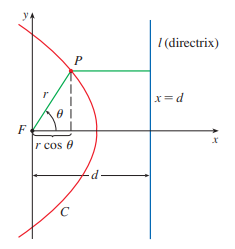
\includegraphics[width=0.26\textwidth]{graph60.png}
\end{wrapfigure}

To derive a polar equation, we place the focus $F$ at the origin (the pole) and the directrix parallel to the y-axis and $d$ units to the right, so its equation is $x=d$. 
\\For any point $P$ with polar coordinates $(r, \theta)$:\\
The distance from the focus $F$ (origin) to $P$ is $|PF| = r$.\\
The distance from $P$ to the directrix $l$ is $|Pl| = d - r \cos\theta$.\\
The defining condition $|PF| = e|Pl|$ is $r = e(d - r \cos\theta)$\\

Squaring both sides of this polar equation and converting to rectangular coordinates, we get:
\begin{align*}
    x^2 + y^2 &= e^2(d - x)^2 = e^2(d^2 - 2dx + x^2) \\
    \Rightarrow (1 - e^2)x^2 + 2de^2x + y^2 &= e^2d^2
\end{align*}

After completing the square, we have:
\[
\left(x + \dfrac{e^2d}{1 - e^2}\right)^2 + \dfrac{y^2}{1 - e^2} = \dfrac{e^2d^2}{(1 - e^2)^2}
\]

If $e < 1$, we recognize this as the equation of an ellipse:
\[
\dfrac{(x - h)^2}{a^2} + \dfrac{y^2}{b^2} = 1
\]
where:
\[
h = -\dfrac{e^2d}{1 - e^2}, \quad a^2 = \dfrac{e^2d^2}{(1 - e^2)^2}, \quad b^2 = \dfrac{e^2d^2}{1 - e^2}
\]
From Section 10.5, the foci of an ellipse are at a distance $c$ from the center, where:
\[
c^2 = a^2 - b^2 = \dfrac{e^4d^2}{(1 - e^2)^2}
\]
This shows that:
\[
c = \dfrac{e^2d}{1 - e^2} = -h
\]
Solving for $r$ from Equation (1), we get:
\[
r(1 + e \cos\theta) = ed \Rightarrow r = \dfrac{ed}{1 + e \cos\theta}
\]
This equation shows how the shape of the conic depends on the eccentricity $e$.

\section*{Polar Equations of Conics}
\begin{tcolorbox}[
    colback=white!,   % 배경색 (빨간색 5%)
    colframe=orange!80!white, % 테두리색 (빨간색 75% + 검은색 25%)
    title=Conics Defined by polar coordinates,   % 제목
    boxrule=0.5mm,          % 테두리 두께
    arc=3mm               % 모서리 둥글기
    ]
    A polar equation of the form
    \[
    r = \dfrac{ed}{1 \pm e \cos\theta} \quad \text{or} \quad r = \dfrac{ed}{1 \pm e \sin\theta}
    \]
    represents a conic section with eccentricity $e$.\\ 
    The conic is an ellipse if $e < 1$, a parabola if $e = 1$, or a hyperbola if $e > 1$.
\end{tcolorbox}

The orientation of the conic is determined by the trigonometric function and the sign in the denominator:

\begin{figure}[htbp]
    \centering
    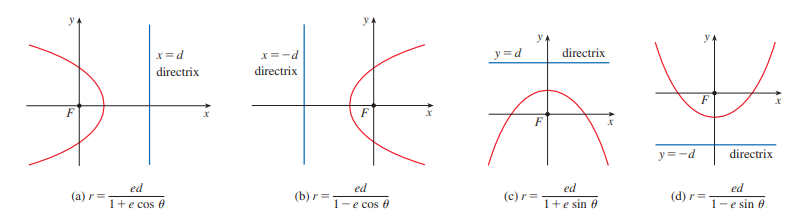
\includegraphics[width=1\textwidth]{graph 61.png}
\end{figure}

\begin{itemize}
    \item[(a)] $1 + e \cos\theta$: Directrix $x = d$ (to the right of the focus)
    \item[(b)] $1 - e \cos\theta$: Directrix $x = -d$ (to the left of the focus)
    \item[(c)] $1 + e \sin\theta$: Directrix $y = d$ (above the focus)
    \item[(d)] $1 - e \sin\theta$: Directrix $y = -d$ (below the focus)
\end{itemize}

\subsection*{EXAMPLE 1}
Find a polar equation for a parabola that has its focus at the origin and whose directrix is the line $y = -6$.\\
\textbf{SOLUTION:}
Using Theorem 6, we have a parabola, so the eccentricity is $e = 1$. The directrix is $y = -6$, so we use the form $r = \dfrac{ed}{1 - e \sin\theta}$ with $d = 6$. The equation is:
\[
r = \dfrac{6}{1 - \sin\theta}
\]

\subsection*{EXAMPLE 2}
A conic is given by the polar equation $r = \dfrac{10}{3 - 2 \cos\theta}$. Find the eccentricity, identify the conic, locate the directrix, and sketch the conic.\\
\textbf{SOLUTION:}
First, we write the equation in the standard form by dividing the numerator and denominator by 3:
\[
r = \dfrac{10/3}{1 - \dfrac{2}{3} \cos\theta}
\]
Comparing this to the standard forms in Theorem 6, we can identify:\\
Eccentricity $e = 2/3$ Conic Identification: Since $e < 1$, the conic is an ellipse.\\
Directrix: The equation is in the form with $1 - e \cos\theta$, which corresponds to a directrix $x = -d$. We have $ed = 10/3$, so $d = (10/3) / (2/3) = 5$. The directrix is the line $x = -5$.
\begin{figure}[htbp]
    \centering
    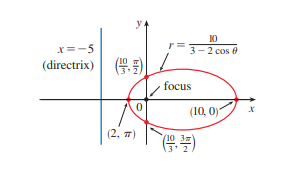
\includegraphics[width=0.4\textwidth]{graph62.png}
\end{figure}

\subsection*{EXAMPLE 3}
Sketch the conic $r = \dfrac{12}{2 + 4 \sin\theta}$.\\
\textbf{SOLUTION:}
First, write the equation in standard form by dividing by 2:
$r = \dfrac{6}{1 + 2 \sin\theta}$\\
Eccentricity:$e = 2$ Conic Identification: Since $e > 1$, the conic is a hyperbola.\\
Directrix:The form is $1 + e \sin\theta$, so the directrix is $y = d$.\\
We have $ed = 6$, so $d = 3$. The directrix is $y = 3$.\\
Asymptotes occur when the denominator is zero: $1 + 2 \sin\theta = 0 \Rightarrow \sin\theta = -1/2$, which occurs at $\theta = 7\pi/6$ and $11\pi/6$.
\begin{figure}[htbp]
    \centering
    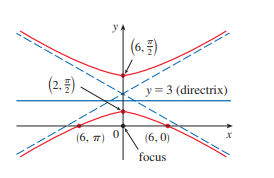
\includegraphics[width=0.3\textwidth]{graph63.png}
\end{figure}

\subsection*{EXAMPLE 4}
If the ellipse of Example 2 is rotated through an angle $\pi/4$ about the origin, find a polar equation and graph the resulting ellipse.\\
\textbf{SOLUTION:}
To rotate a curve through an angle $\alpha$, we replace $\theta$ with $(\theta - \alpha)$ in its polar equation. The original equation is $r = \dfrac{10}{3 - 2 \cos\theta}$.\\
Replacing $\theta$ with $(\theta - \pi/4)$, the new equation is:
$r = \dfrac{10}{3 - 2 \cos(\theta - \pi/4)}$\\
The graph is the ellipse from Example 2, rotated counterclockwise by $\pi/4$ about its left focus (the origin).
\begin{figure}[htbp]
    \centering
    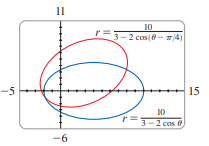
\includegraphics[width=0.3\textwidth]{graph64.png}
\end{figure}

\section*{Kepler's Laws and Planetary Motion}
In 1609, Johannes Kepler formulated three laws of planetary motion based on astronomical data.
\begin{tcolorbox}[
    colback=white!,   % 배경색 (빨간색 5%)
    colframe=orange!80!white, % 테두리색 (빨간색 75% + 검은색 25%)
    title=Kepler's Laws,   % 제목
    boxrule=0.5mm,          % 테두리 두께
    arc=3mm               % 모서리 둥글기
    ]
    \begin{enumerate}
        \item A planet revolves around the sun in an elliptical orbit with the sun at one focus.
        \item The line joining the sun to a planet sweeps out equal areas in equal times.
        \item The square of the period of revolution of a planet is proportional to the cube of the length of the major axis of its orbit.
    \end{enumerate}
\end{tcolorbox}

\begin{figure}[htbp]
    \centering
    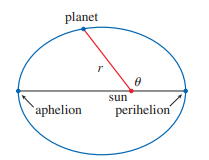
\includegraphics[width=0.3\textwidth]{graph65.png}
\end{figure}
For astronomical calculations, the polar equation of an ellipse can be expressed in terms of its semimajor axis $a$ and eccentricity $e$.\\
Polar Equation of an Elliptical Orbit :  \[
    r = \dfrac{a(1 - e^2)}{1 + e \cos\theta}
    \]
This equation describes an ellipse with the sun at the focus (origin), semimajor axis $a$, and eccentricity $e$.
The points in the orbit closest to and farthest from the sun are the perihelion and aphelion, respectively.

\begin{tcolorbox}[
    colback=white!,   % 배경색 (빨간색 5%)
    colframe=orange!80!white, % 테두리색 (빨간색 75% + 검은색 25%)
    title=,   % 제목
    boxrule=0.5mm,      % 테두리 두께
    arc=3mm          % 모서리 둥글기
    ]
    \begin{itemize}
        \item[-] Perihelion distance ($\theta = 0$): $r = a(1 - e)$
        \item[-] Aphelion distance ($\theta = \pi$): $r = a(1 + e)$
    \end{itemize}
\end{tcolorbox}


\subsection*{EXAMPLE 5}
(a) Find an approximate polar equation for the elliptical orbit of the Earth around the Sun (at one focus) given that the eccentricity is about $0.017$ and the length of the major axis is about $2.99 \times 10^8$ km.\\
(b) Find the distance from the Earth to the Sun at perihelion and at aphelion.\\
\textbf{SOLUTION:}\\
(a) The length of the major axis is $2a = 2.99 \times 10^8$ km, so the semimajor axis is $a = 1.495 \times 10^8$ km. The eccentricity is $e = 0.017$.\\
Using the polar equation:
\[
r = \dfrac{a(1 - e^2)}{1 + e \cos\theta} = \dfrac{1.495 \times 10^8 (1 - 0.017^2)}{1 + 0.017 \cos\theta} \approx \dfrac{1.49 \times 10^8}{1 + 0.017 \cos\theta}
\]
(b) Perihelion distance: $a(1 - e) \approx (1.495 \times 10^8)(1 - 0.017) \approx 1.47 \times 10^8$ km \\
 Aphelion distance: $a(1 + e) \approx (1.495 \times 10^8)(1 + 0.017) \approx 1.52 \times 10^8$ km

\end{document}

